\begin{figure}[h]
	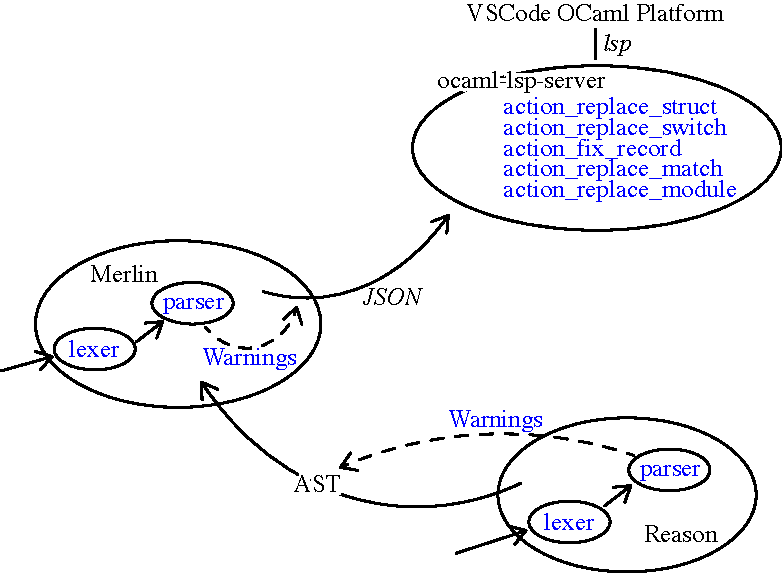
\includegraphics[width=\linewidth]{graph.pdf}
\caption{Архитектура расширения. Стрелки обозначают передачу данных. Курсивом выделены протоколы. Синим цветом выделены части, которые подверглись изменениям, зелёным~--- новые модули.}
\end{figure}
Поддержка OCaml в Reason реализована через новые синтаксические правила для парсера. Для этих правил так же созданы предупреждения (warnings), как новый тип reason\_warning, по примеру существующего в Reason типа reason\_error. Во время работы парсера предупреждения выкидываются из него и собираются. Далее они, с помощью добавленной функции warning\_attribute, превращаются в атрибуты AST и вместе с ним передаются в merlin, откуда идут в ocaml-lsp и в итоге в IDE. Необходимая поддержка атрибутов reason.warning добавлена на стороне merlin.

Поддержка Reason в OCaml реализована через новые правила для парсера и расширение стандартного списка предупреждений OCaml.

Стоит заметить, что для Reason реализована поддержка второго языка как при {\it компиляции}, так и в {\it IDE}, тогда как у OCaml только для {\it IDE}. Такая ситуация возникла из-за того, что у Reason одна кодовая база для парсера, компилятора и reason-merlin, в отличии от OCaml, где два разных репозитория для компилятора и Merlin. В нашем случае частичная поддержка Reason была добавлена только в Merlin.

Функции исправления кода в ocaml-lsp как для Reason, так и для OCaml созданы по примеру action\_add\_rec\footnote{ \url{https://github.com/ocaml/ocaml-lsp/blob/1.13.1/ocaml-lsp-server/src/code_actions/action_add_rec.ml} (дата доступа: 24.08.2022) }. Action\_add\_rec~--- это code\-Action, добавляющий слово {\it rec} перед рекурсивной функцией, если его ещё не было. CodeAction, являющийся частью спецификации протокола lsp, представляет собой изменение, которое может быть выполнено в коде, например для рефакторинга кода.
\newpage
